% Copyright © 2013 Martin Ueding <dev@martin-ueding.de>
%
% Copyright © 2012-2013 Martin Ueding <dev@martin-ueding.de>

% This is my general purpose LaTeX header file for writing German documents.
% Ideally, you include this using a simple ``% Copyright © 2012-2013 Martin Ueding <dev@martin-ueding.de>

% This is my general purpose LaTeX header file for writing German documents.
% Ideally, you include this using a simple ``% Copyright © 2012-2013 Martin Ueding <dev@martin-ueding.de>

% This is my general purpose LaTeX header file for writing German documents.
% Ideally, you include this using a simple ``\input{header.tex}`` in your main
% document and start with ``\title`` and ``\begin{document}`` afterwards.

% If you need to add additional packages, I recommend not doing this in this
% file, but in your main document. That way, you can just drop in a new
% ``header.tex`` and get all the new commands without having to merge manually.

% Since this file encorporates a CC-BY-SA fragment, this whole files is
% licensed under the CC-BY-SA license.

\documentclass[11pt, ngerman, fleqn, DIV=15, headinclude]{scrartcl}

\usepackage{graphicx}

% Environment to quote the problem. Currently, this is just a new name for the
% quote environment.
\newenvironment{problem}{\begin{quote}}{\end{quote}}

%%%%%%%%%%%%%%%%%%%%%%%%%%%%%%%%%%%%%%%%%%%%%%%%%%%%%%%%%%%%%%%%%%%%%%%%%%%%%%%
%                                Locale, date                                 %
%%%%%%%%%%%%%%%%%%%%%%%%%%%%%%%%%%%%%%%%%%%%%%%%%%%%%%%%%%%%%%%%%%%%%%%%%%%%%%%

\usepackage{babel}
\usepackage[iso]{isodate}

%%%%%%%%%%%%%%%%%%%%%%%%%%%%%%%%%%%%%%%%%%%%%%%%%%%%%%%%%%%%%%%%%%%%%%%%%%%%%%%
%                          Margins and other spacing                          %
%%%%%%%%%%%%%%%%%%%%%%%%%%%%%%%%%%%%%%%%%%%%%%%%%%%%%%%%%%%%%%%%%%%%%%%%%%%%%%%

\usepackage[parfill]{parskip}
\usepackage{setspace}
\usepackage[activate]{microtype}

\setlength{\columnsep}{2cm}

%%%%%%%%%%%%%%%%%%%%%%%%%%%%%%%%%%%%%%%%%%%%%%%%%%%%%%%%%%%%%%%%%%%%%%%%%%%%%%%
%                                    Color                                    %
%%%%%%%%%%%%%%%%%%%%%%%%%%%%%%%%%%%%%%%%%%%%%%%%%%%%%%%%%%%%%%%%%%%%%%%%%%%%%%%

\usepackage[usenames, dvipsnames]{xcolor}

\colorlet{darkred}{red!70!black}
\colorlet{darkblue}{blue!70!black}
\colorlet{darkgreen}{green!40!black}

%%%%%%%%%%%%%%%%%%%%%%%%%%%%%%%%%%%%%%%%%%%%%%%%%%%%%%%%%%%%%%%%%%%%%%%%%%%%%%%
%                         Font and font like settings                         %
%%%%%%%%%%%%%%%%%%%%%%%%%%%%%%%%%%%%%%%%%%%%%%%%%%%%%%%%%%%%%%%%%%%%%%%%%%%%%%%

% This replaces all fonts with Bitstream Charter, Bitstream Vera Sans and
% Bitstream Vera Mono. Math will be rendered in Charter.
\usepackage[charter, greekuppercase=italicized]{mathdesign}
\usepackage{beramono}
\usepackage{berasans}

% Bold, sans-serif tensors. This fragment is taken from “egreg” from
% http://tex.stackexchange.com/a/82747/8945 and licensed under `CC-BY-SA
% <https://creativecommons.org/licenses/by-sa/3.0/>`_.
\usepackage{bm}
\DeclareMathAlphabet{\mathsfit}{\encodingdefault}{\sfdefault}{m}{sl}
\SetMathAlphabet{\mathsfit}{bold}{\encodingdefault}{\sfdefault}{bx}{sl}
\newcommand{\tens}[1]{\bm{\mathsfit{#1}}}

% Bold vectors.
\renewcommand{\vec}[1]{\boldsymbol{#1}}

%%%%%%%%%%%%%%%%%%%%%%%%%%%%%%%%%%%%%%%%%%%%%%%%%%%%%%%%%%%%%%%%%%%%%%%%%%%%%%%
%                               Input encoding                                %
%%%%%%%%%%%%%%%%%%%%%%%%%%%%%%%%%%%%%%%%%%%%%%%%%%%%%%%%%%%%%%%%%%%%%%%%%%%%%%%

\usepackage[T1]{fontenc}
\usepackage[utf8]{inputenc}

%%%%%%%%%%%%%%%%%%%%%%%%%%%%%%%%%%%%%%%%%%%%%%%%%%%%%%%%%%%%%%%%%%%%%%%%%%%%%%%
%                         Hyperrefs and PDF metadata                          %
%%%%%%%%%%%%%%%%%%%%%%%%%%%%%%%%%%%%%%%%%%%%%%%%%%%%%%%%%%%%%%%%%%%%%%%%%%%%%%%

\usepackage{hyperref}
\usepackage{lastpage}

% This sets the author in the properties of the PDF as well. If you want to
% change it, just override it with another ``\hypersetup`` call.
\hypersetup{
	breaklinks=false,
	citecolor=darkgreen,
	colorlinks=true,
	linkcolor=darkblue,
	menucolor=black,
	pdfauthor={Martin Ueding},
	urlcolor=darkblue,
}

%%%%%%%%%%%%%%%%%%%%%%%%%%%%%%%%%%%%%%%%%%%%%%%%%%%%%%%%%%%%%%%%%%%%%%%%%%%%%%%
%                               Math Operators                                %
%%%%%%%%%%%%%%%%%%%%%%%%%%%%%%%%%%%%%%%%%%%%%%%%%%%%%%%%%%%%%%%%%%%%%%%%%%%%%%%

% AMS environments like ``align`` and theorems like ``proof``.
\usepackage{amsmath}
\usepackage{amsthm}

% Common math constructs like partial derivatives.
\usepackage{commath}

% Physical units.
\usepackage[output-decimal-marker={,}]{siunitx}

% Word like operators.
\DeclareMathOperator{\acosh}{arcosh}
\DeclareMathOperator{\arcosh}{arcosh}
\DeclareMathOperator{\arcsinh}{arsinh}
\DeclareMathOperator{\arsinh}{arsinh}
\DeclareMathOperator{\asinh}{arsinh}
\DeclareMathOperator{\card}{card}
\DeclareMathOperator{\csch}{cshs}
\DeclareMathOperator{\diam}{diam}
\DeclareMathOperator{\sech}{sech}
\renewcommand{\Im}{\mathop{{}\mathrm{Im}}\nolimits}
\renewcommand{\Re}{\mathop{{}\mathrm{Re}}\nolimits}

% Fourier transform.
\DeclareMathOperator{\fourier}{\ensuremath{\mathcal{F}}}

% Roman versions of “e” and “i” to serve as Euler's number and the imaginary
% constant.
\newcommand{\ee}{\eup}
\newcommand{\eup}{\mathrm e}
\newcommand{\ii}{\iup}
\newcommand{\iup}{\mathrm i}

% Symbols for the various mathematical fields (natural numbers, integers,
% rational numbers, real numbers, complex numbers).
\newcommand{\C}{\ensuremath{\mathbb C}}
\newcommand{\N}{\ensuremath{\mathbb N}}
\newcommand{\Q}{\ensuremath{\mathbb Q}}
\newcommand{\R}{\ensuremath{\mathbb R}}
\newcommand{\Z}{\ensuremath{\mathbb Z}}

% Shape like operators.
\DeclareMathOperator{\dalambert}{\Box}
\DeclareMathOperator{\laplace}{\bigtriangleup}
\newcommand{\curl}{\vnabla \times}
\newcommand{\divergence}[1]{\inner{\vnabla}{#1}}
\newcommand{\vnabla}{\vec \nabla}

\newcommand{\half}{\frac 12}

% Unit vector (German „Einheitsvektor“).
\newcommand{\ev}{\hat{\vec e}}

% Scientific notation for large numbers.
\newcommand{\e}[1]{\cdot 10^{#1}}

% Mathematician's notation for the inner (scalar, dot) product.
\newcommand{\bracket}[1]{\left\langle #1 \right\rangle}
\newcommand{\inner}[2]{\bracket{#1, #2}}

% Placeholders.
\newcommand{\emesswert}{\del{\messwert \pm \messwert}}
\newcommand{\fehlt}{\textcolor{darkred}{Hier fehlen noch Inhalte.}}
\newcommand{\messwert}{\textcolor{blue}{\square}}
\newcommand{\punkte}{\phantom{xxxxx}}
\newcommand{\punktevon}[1]{\begin{flushright}/ #1\end{flushright}}

% Separator for equations on a single line.
\newcommand{\eqnsep}{,\quad}

% Quantum Mechanics
\newcommand{\braket}[2]{\left\langle #1 \left. \vphantom{#1 #2} \right| #2 \right\rangle}
\newcommand{\braopket}[3]{\left\langle #1 \left. \vphantom{#1 #2 #3} \right| #2 \left. \vphantom{#1 #2 #3} \right| #3 \right\rangle}
\newcommand{\bra}[1]{\left\langle #1 \right|}
\newcommand{\ketbra}[2]{\left| #1 \vphantom{#2} \right\rangle \left\langle #2  \vphantom{#1} \right|}
\newcommand{\ket}[1]{\left| #1 \right\rangle}

%%%%%%%%%%%%%%%%%%%%%%%%%%%%%%%%%%%%%%%%%%%%%%%%%%%%%%%%%%%%%%%%%%%%%%%%%%%%%%%
%                                  Headings                                   %
%%%%%%%%%%%%%%%%%%%%%%%%%%%%%%%%%%%%%%%%%%%%%%%%%%%%%%%%%%%%%%%%%%%%%%%%%%%%%%%

% This will set fancy headings to the top of the page. The page number will be
% accompanied by the total number of pages. That way, you will know if any page
% is missing.
%
% If you do not want this for your document, you can just use
% ``\pagestyle{plain}``.

\usepackage{scrpage2}

\pagestyle{scrheadings}
\automark{section}
\cfoot{\footnotesize{Seite \thepage\ / \pageref{LastPage}}}
\chead{}
\ihead{}
\ohead{\rightmark}
\setheadsepline{.4pt}

%%%%%%%%%%%%%%%%%%%%%%%%%%%%%%%%%%%%%%%%%%%%%%%%%%%%%%%%%%%%%%%%%%%%%%%%%%%%%%%
%                            Bibliography (BibTeX)                            %
%%%%%%%%%%%%%%%%%%%%%%%%%%%%%%%%%%%%%%%%%%%%%%%%%%%%%%%%%%%%%%%%%%%%%%%%%%%%%%%

\newcommand{\bibliographyfile}{../../zentrale_BibTeX/Central}
\bibliographystyle{apalike2}

%%%%%%%%%%%%%%%%%%%%%%%%%%%%%%%%%%%%%%%%%%%%%%%%%%%%%%%%%%%%%%%%%%%%%%%%%%%%%%%
%                                Abbreviations                                %
%%%%%%%%%%%%%%%%%%%%%%%%%%%%%%%%%%%%%%%%%%%%%%%%%%%%%%%%%%%%%%%%%%%%%%%%%%%%%%%

\newcommand{\dhabk}{\mbox{d.\,h.}}

%%%%%%%%%%%%%%%%%%%%%%%%%%%%%%%%%%%%%%%%%%%%%%%%%%%%%%%%%%%%%%%%%%%%%%%%%%%%%%%
%                                  Licences                                   %
%%%%%%%%%%%%%%%%%%%%%%%%%%%%%%%%%%%%%%%%%%%%%%%%%%%%%%%%%%%%%%%%%%%%%%%%%%%%%%%

\usepackage{ccicons}

\newcommand{\ccbysadetext}{%
	\begin{small}
		Dieses Werk bzw. Inhalt steht unter einer
		\href{http://creativecommons.org/licenses/by-sa/3.0/deed.de}{%
			Creative Commons Namensnennung - Weitergabe unter gleichen
		Bedingungen 3.0 Unported Lizenz}.
	\end{small}
}

\newcommand{\ccbysadetitle}{%
	Lizenz: \href{http://creativecommons.org/licenses/by-sa/3.0/deed.de}
	{CC-BY-SA 3.0 \ccbysa}
}
`` in your main
% document and start with ``\title`` and ``\begin{document}`` afterwards.

% If you need to add additional packages, I recommend not doing this in this
% file, but in your main document. That way, you can just drop in a new
% ``header.tex`` and get all the new commands without having to merge manually.

% Since this file encorporates a CC-BY-SA fragment, this whole files is
% licensed under the CC-BY-SA license.

\documentclass[11pt, ngerman, fleqn, DIV=15, headinclude]{scrartcl}

\usepackage{graphicx}

% Environment to quote the problem. Currently, this is just a new name for the
% quote environment.
\newenvironment{problem}{\begin{quote}}{\end{quote}}

%%%%%%%%%%%%%%%%%%%%%%%%%%%%%%%%%%%%%%%%%%%%%%%%%%%%%%%%%%%%%%%%%%%%%%%%%%%%%%%
%                                Locale, date                                 %
%%%%%%%%%%%%%%%%%%%%%%%%%%%%%%%%%%%%%%%%%%%%%%%%%%%%%%%%%%%%%%%%%%%%%%%%%%%%%%%

\usepackage{babel}
\usepackage[iso]{isodate}

%%%%%%%%%%%%%%%%%%%%%%%%%%%%%%%%%%%%%%%%%%%%%%%%%%%%%%%%%%%%%%%%%%%%%%%%%%%%%%%
%                          Margins and other spacing                          %
%%%%%%%%%%%%%%%%%%%%%%%%%%%%%%%%%%%%%%%%%%%%%%%%%%%%%%%%%%%%%%%%%%%%%%%%%%%%%%%

\usepackage[parfill]{parskip}
\usepackage{setspace}
\usepackage[activate]{microtype}

\setlength{\columnsep}{2cm}

%%%%%%%%%%%%%%%%%%%%%%%%%%%%%%%%%%%%%%%%%%%%%%%%%%%%%%%%%%%%%%%%%%%%%%%%%%%%%%%
%                                    Color                                    %
%%%%%%%%%%%%%%%%%%%%%%%%%%%%%%%%%%%%%%%%%%%%%%%%%%%%%%%%%%%%%%%%%%%%%%%%%%%%%%%

\usepackage[usenames, dvipsnames]{xcolor}

\colorlet{darkred}{red!70!black}
\colorlet{darkblue}{blue!70!black}
\colorlet{darkgreen}{green!40!black}

%%%%%%%%%%%%%%%%%%%%%%%%%%%%%%%%%%%%%%%%%%%%%%%%%%%%%%%%%%%%%%%%%%%%%%%%%%%%%%%
%                         Font and font like settings                         %
%%%%%%%%%%%%%%%%%%%%%%%%%%%%%%%%%%%%%%%%%%%%%%%%%%%%%%%%%%%%%%%%%%%%%%%%%%%%%%%

% This replaces all fonts with Bitstream Charter, Bitstream Vera Sans and
% Bitstream Vera Mono. Math will be rendered in Charter.
\usepackage[charter, greekuppercase=italicized]{mathdesign}
\usepackage{beramono}
\usepackage{berasans}

% Bold, sans-serif tensors. This fragment is taken from “egreg” from
% http://tex.stackexchange.com/a/82747/8945 and licensed under `CC-BY-SA
% <https://creativecommons.org/licenses/by-sa/3.0/>`_.
\usepackage{bm}
\DeclareMathAlphabet{\mathsfit}{\encodingdefault}{\sfdefault}{m}{sl}
\SetMathAlphabet{\mathsfit}{bold}{\encodingdefault}{\sfdefault}{bx}{sl}
\newcommand{\tens}[1]{\bm{\mathsfit{#1}}}

% Bold vectors.
\renewcommand{\vec}[1]{\boldsymbol{#1}}

%%%%%%%%%%%%%%%%%%%%%%%%%%%%%%%%%%%%%%%%%%%%%%%%%%%%%%%%%%%%%%%%%%%%%%%%%%%%%%%
%                               Input encoding                                %
%%%%%%%%%%%%%%%%%%%%%%%%%%%%%%%%%%%%%%%%%%%%%%%%%%%%%%%%%%%%%%%%%%%%%%%%%%%%%%%

\usepackage[T1]{fontenc}
\usepackage[utf8]{inputenc}

%%%%%%%%%%%%%%%%%%%%%%%%%%%%%%%%%%%%%%%%%%%%%%%%%%%%%%%%%%%%%%%%%%%%%%%%%%%%%%%
%                         Hyperrefs and PDF metadata                          %
%%%%%%%%%%%%%%%%%%%%%%%%%%%%%%%%%%%%%%%%%%%%%%%%%%%%%%%%%%%%%%%%%%%%%%%%%%%%%%%

\usepackage{hyperref}
\usepackage{lastpage}

% This sets the author in the properties of the PDF as well. If you want to
% change it, just override it with another ``\hypersetup`` call.
\hypersetup{
	breaklinks=false,
	citecolor=darkgreen,
	colorlinks=true,
	linkcolor=darkblue,
	menucolor=black,
	pdfauthor={Martin Ueding},
	urlcolor=darkblue,
}

%%%%%%%%%%%%%%%%%%%%%%%%%%%%%%%%%%%%%%%%%%%%%%%%%%%%%%%%%%%%%%%%%%%%%%%%%%%%%%%
%                               Math Operators                                %
%%%%%%%%%%%%%%%%%%%%%%%%%%%%%%%%%%%%%%%%%%%%%%%%%%%%%%%%%%%%%%%%%%%%%%%%%%%%%%%

% AMS environments like ``align`` and theorems like ``proof``.
\usepackage{amsmath}
\usepackage{amsthm}

% Common math constructs like partial derivatives.
\usepackage{commath}

% Physical units.
\usepackage[output-decimal-marker={,}]{siunitx}

% Word like operators.
\DeclareMathOperator{\acosh}{arcosh}
\DeclareMathOperator{\arcosh}{arcosh}
\DeclareMathOperator{\arcsinh}{arsinh}
\DeclareMathOperator{\arsinh}{arsinh}
\DeclareMathOperator{\asinh}{arsinh}
\DeclareMathOperator{\card}{card}
\DeclareMathOperator{\csch}{cshs}
\DeclareMathOperator{\diam}{diam}
\DeclareMathOperator{\sech}{sech}
\renewcommand{\Im}{\mathop{{}\mathrm{Im}}\nolimits}
\renewcommand{\Re}{\mathop{{}\mathrm{Re}}\nolimits}

% Fourier transform.
\DeclareMathOperator{\fourier}{\ensuremath{\mathcal{F}}}

% Roman versions of “e” and “i” to serve as Euler's number and the imaginary
% constant.
\newcommand{\ee}{\eup}
\newcommand{\eup}{\mathrm e}
\newcommand{\ii}{\iup}
\newcommand{\iup}{\mathrm i}

% Symbols for the various mathematical fields (natural numbers, integers,
% rational numbers, real numbers, complex numbers).
\newcommand{\C}{\ensuremath{\mathbb C}}
\newcommand{\N}{\ensuremath{\mathbb N}}
\newcommand{\Q}{\ensuremath{\mathbb Q}}
\newcommand{\R}{\ensuremath{\mathbb R}}
\newcommand{\Z}{\ensuremath{\mathbb Z}}

% Shape like operators.
\DeclareMathOperator{\dalambert}{\Box}
\DeclareMathOperator{\laplace}{\bigtriangleup}
\newcommand{\curl}{\vnabla \times}
\newcommand{\divergence}[1]{\inner{\vnabla}{#1}}
\newcommand{\vnabla}{\vec \nabla}

\newcommand{\half}{\frac 12}

% Unit vector (German „Einheitsvektor“).
\newcommand{\ev}{\hat{\vec e}}

% Scientific notation for large numbers.
\newcommand{\e}[1]{\cdot 10^{#1}}

% Mathematician's notation for the inner (scalar, dot) product.
\newcommand{\bracket}[1]{\left\langle #1 \right\rangle}
\newcommand{\inner}[2]{\bracket{#1, #2}}

% Placeholders.
\newcommand{\emesswert}{\del{\messwert \pm \messwert}}
\newcommand{\fehlt}{\textcolor{darkred}{Hier fehlen noch Inhalte.}}
\newcommand{\messwert}{\textcolor{blue}{\square}}
\newcommand{\punkte}{\phantom{xxxxx}}
\newcommand{\punktevon}[1]{\begin{flushright}/ #1\end{flushright}}

% Separator for equations on a single line.
\newcommand{\eqnsep}{,\quad}

% Quantum Mechanics
\newcommand{\braket}[2]{\left\langle #1 \left. \vphantom{#1 #2} \right| #2 \right\rangle}
\newcommand{\braopket}[3]{\left\langle #1 \left. \vphantom{#1 #2 #3} \right| #2 \left. \vphantom{#1 #2 #3} \right| #3 \right\rangle}
\newcommand{\bra}[1]{\left\langle #1 \right|}
\newcommand{\ketbra}[2]{\left| #1 \vphantom{#2} \right\rangle \left\langle #2  \vphantom{#1} \right|}
\newcommand{\ket}[1]{\left| #1 \right\rangle}

%%%%%%%%%%%%%%%%%%%%%%%%%%%%%%%%%%%%%%%%%%%%%%%%%%%%%%%%%%%%%%%%%%%%%%%%%%%%%%%
%                                  Headings                                   %
%%%%%%%%%%%%%%%%%%%%%%%%%%%%%%%%%%%%%%%%%%%%%%%%%%%%%%%%%%%%%%%%%%%%%%%%%%%%%%%

% This will set fancy headings to the top of the page. The page number will be
% accompanied by the total number of pages. That way, you will know if any page
% is missing.
%
% If you do not want this for your document, you can just use
% ``\pagestyle{plain}``.

\usepackage{scrpage2}

\pagestyle{scrheadings}
\automark{section}
\cfoot{\footnotesize{Seite \thepage\ / \pageref{LastPage}}}
\chead{}
\ihead{}
\ohead{\rightmark}
\setheadsepline{.4pt}

%%%%%%%%%%%%%%%%%%%%%%%%%%%%%%%%%%%%%%%%%%%%%%%%%%%%%%%%%%%%%%%%%%%%%%%%%%%%%%%
%                            Bibliography (BibTeX)                            %
%%%%%%%%%%%%%%%%%%%%%%%%%%%%%%%%%%%%%%%%%%%%%%%%%%%%%%%%%%%%%%%%%%%%%%%%%%%%%%%

\newcommand{\bibliographyfile}{../../zentrale_BibTeX/Central}
\bibliographystyle{apalike2}

%%%%%%%%%%%%%%%%%%%%%%%%%%%%%%%%%%%%%%%%%%%%%%%%%%%%%%%%%%%%%%%%%%%%%%%%%%%%%%%
%                                Abbreviations                                %
%%%%%%%%%%%%%%%%%%%%%%%%%%%%%%%%%%%%%%%%%%%%%%%%%%%%%%%%%%%%%%%%%%%%%%%%%%%%%%%

\newcommand{\dhabk}{\mbox{d.\,h.}}

%%%%%%%%%%%%%%%%%%%%%%%%%%%%%%%%%%%%%%%%%%%%%%%%%%%%%%%%%%%%%%%%%%%%%%%%%%%%%%%
%                                  Licences                                   %
%%%%%%%%%%%%%%%%%%%%%%%%%%%%%%%%%%%%%%%%%%%%%%%%%%%%%%%%%%%%%%%%%%%%%%%%%%%%%%%

\usepackage{ccicons}

\newcommand{\ccbysadetext}{%
	\begin{small}
		Dieses Werk bzw. Inhalt steht unter einer
		\href{http://creativecommons.org/licenses/by-sa/3.0/deed.de}{%
			Creative Commons Namensnennung - Weitergabe unter gleichen
		Bedingungen 3.0 Unported Lizenz}.
	\end{small}
}

\newcommand{\ccbysadetitle}{%
	Lizenz: \href{http://creativecommons.org/licenses/by-sa/3.0/deed.de}
	{CC-BY-SA 3.0 \ccbysa}
}
`` in your main
% document and start with ``\title`` and ``\begin{document}`` afterwards.

% If you need to add additional packages, I recommend not doing this in this
% file, but in your main document. That way, you can just drop in a new
% ``header.tex`` and get all the new commands without having to merge manually.

% Since this file encorporates a CC-BY-SA fragment, this whole files is
% licensed under the CC-BY-SA license.

\documentclass[11pt, ngerman, fleqn, DIV=15, headinclude]{scrartcl}

\usepackage{graphicx}

% Environment to quote the problem. Currently, this is just a new name for the
% quote environment.
\newenvironment{problem}{\begin{quote}}{\end{quote}}

%%%%%%%%%%%%%%%%%%%%%%%%%%%%%%%%%%%%%%%%%%%%%%%%%%%%%%%%%%%%%%%%%%%%%%%%%%%%%%%
%                                Locale, date                                 %
%%%%%%%%%%%%%%%%%%%%%%%%%%%%%%%%%%%%%%%%%%%%%%%%%%%%%%%%%%%%%%%%%%%%%%%%%%%%%%%

\usepackage{babel}
\usepackage[iso]{isodate}

%%%%%%%%%%%%%%%%%%%%%%%%%%%%%%%%%%%%%%%%%%%%%%%%%%%%%%%%%%%%%%%%%%%%%%%%%%%%%%%
%                          Margins and other spacing                          %
%%%%%%%%%%%%%%%%%%%%%%%%%%%%%%%%%%%%%%%%%%%%%%%%%%%%%%%%%%%%%%%%%%%%%%%%%%%%%%%

\usepackage[parfill]{parskip}
\usepackage{setspace}
\usepackage[activate]{microtype}

\setlength{\columnsep}{2cm}

%%%%%%%%%%%%%%%%%%%%%%%%%%%%%%%%%%%%%%%%%%%%%%%%%%%%%%%%%%%%%%%%%%%%%%%%%%%%%%%
%                                    Color                                    %
%%%%%%%%%%%%%%%%%%%%%%%%%%%%%%%%%%%%%%%%%%%%%%%%%%%%%%%%%%%%%%%%%%%%%%%%%%%%%%%

\usepackage[usenames, dvipsnames]{xcolor}

\colorlet{darkred}{red!70!black}
\colorlet{darkblue}{blue!70!black}
\colorlet{darkgreen}{green!40!black}

%%%%%%%%%%%%%%%%%%%%%%%%%%%%%%%%%%%%%%%%%%%%%%%%%%%%%%%%%%%%%%%%%%%%%%%%%%%%%%%
%                         Font and font like settings                         %
%%%%%%%%%%%%%%%%%%%%%%%%%%%%%%%%%%%%%%%%%%%%%%%%%%%%%%%%%%%%%%%%%%%%%%%%%%%%%%%

% This replaces all fonts with Bitstream Charter, Bitstream Vera Sans and
% Bitstream Vera Mono. Math will be rendered in Charter.
\usepackage[charter, greekuppercase=italicized]{mathdesign}
\usepackage{beramono}
\usepackage{berasans}

% Bold, sans-serif tensors. This fragment is taken from “egreg” from
% http://tex.stackexchange.com/a/82747/8945 and licensed under `CC-BY-SA
% <https://creativecommons.org/licenses/by-sa/3.0/>`_.
\usepackage{bm}
\DeclareMathAlphabet{\mathsfit}{\encodingdefault}{\sfdefault}{m}{sl}
\SetMathAlphabet{\mathsfit}{bold}{\encodingdefault}{\sfdefault}{bx}{sl}
\newcommand{\tens}[1]{\bm{\mathsfit{#1}}}

% Bold vectors.
\renewcommand{\vec}[1]{\boldsymbol{#1}}

%%%%%%%%%%%%%%%%%%%%%%%%%%%%%%%%%%%%%%%%%%%%%%%%%%%%%%%%%%%%%%%%%%%%%%%%%%%%%%%
%                               Input encoding                                %
%%%%%%%%%%%%%%%%%%%%%%%%%%%%%%%%%%%%%%%%%%%%%%%%%%%%%%%%%%%%%%%%%%%%%%%%%%%%%%%

\usepackage[T1]{fontenc}
\usepackage[utf8]{inputenc}

%%%%%%%%%%%%%%%%%%%%%%%%%%%%%%%%%%%%%%%%%%%%%%%%%%%%%%%%%%%%%%%%%%%%%%%%%%%%%%%
%                         Hyperrefs and PDF metadata                          %
%%%%%%%%%%%%%%%%%%%%%%%%%%%%%%%%%%%%%%%%%%%%%%%%%%%%%%%%%%%%%%%%%%%%%%%%%%%%%%%

\usepackage{hyperref}
\usepackage{lastpage}

% This sets the author in the properties of the PDF as well. If you want to
% change it, just override it with another ``\hypersetup`` call.
\hypersetup{
	breaklinks=false,
	citecolor=darkgreen,
	colorlinks=true,
	linkcolor=darkblue,
	menucolor=black,
	pdfauthor={Martin Ueding},
	urlcolor=darkblue,
}

%%%%%%%%%%%%%%%%%%%%%%%%%%%%%%%%%%%%%%%%%%%%%%%%%%%%%%%%%%%%%%%%%%%%%%%%%%%%%%%
%                               Math Operators                                %
%%%%%%%%%%%%%%%%%%%%%%%%%%%%%%%%%%%%%%%%%%%%%%%%%%%%%%%%%%%%%%%%%%%%%%%%%%%%%%%

% AMS environments like ``align`` and theorems like ``proof``.
\usepackage{amsmath}
\usepackage{amsthm}

% Common math constructs like partial derivatives.
\usepackage{commath}

% Physical units.
\usepackage[output-decimal-marker={,}]{siunitx}

% Word like operators.
\DeclareMathOperator{\acosh}{arcosh}
\DeclareMathOperator{\arcosh}{arcosh}
\DeclareMathOperator{\arcsinh}{arsinh}
\DeclareMathOperator{\arsinh}{arsinh}
\DeclareMathOperator{\asinh}{arsinh}
\DeclareMathOperator{\card}{card}
\DeclareMathOperator{\csch}{cshs}
\DeclareMathOperator{\diam}{diam}
\DeclareMathOperator{\sech}{sech}
\renewcommand{\Im}{\mathop{{}\mathrm{Im}}\nolimits}
\renewcommand{\Re}{\mathop{{}\mathrm{Re}}\nolimits}

% Fourier transform.
\DeclareMathOperator{\fourier}{\ensuremath{\mathcal{F}}}

% Roman versions of “e” and “i” to serve as Euler's number and the imaginary
% constant.
\newcommand{\ee}{\eup}
\newcommand{\eup}{\mathrm e}
\newcommand{\ii}{\iup}
\newcommand{\iup}{\mathrm i}

% Symbols for the various mathematical fields (natural numbers, integers,
% rational numbers, real numbers, complex numbers).
\newcommand{\C}{\ensuremath{\mathbb C}}
\newcommand{\N}{\ensuremath{\mathbb N}}
\newcommand{\Q}{\ensuremath{\mathbb Q}}
\newcommand{\R}{\ensuremath{\mathbb R}}
\newcommand{\Z}{\ensuremath{\mathbb Z}}

% Shape like operators.
\DeclareMathOperator{\dalambert}{\Box}
\DeclareMathOperator{\laplace}{\bigtriangleup}
\newcommand{\curl}{\vnabla \times}
\newcommand{\divergence}[1]{\inner{\vnabla}{#1}}
\newcommand{\vnabla}{\vec \nabla}

\newcommand{\half}{\frac 12}

% Unit vector (German „Einheitsvektor“).
\newcommand{\ev}{\hat{\vec e}}

% Scientific notation for large numbers.
\newcommand{\e}[1]{\cdot 10^{#1}}

% Mathematician's notation for the inner (scalar, dot) product.
\newcommand{\bracket}[1]{\left\langle #1 \right\rangle}
\newcommand{\inner}[2]{\bracket{#1, #2}}

% Placeholders.
\newcommand{\emesswert}{\del{\messwert \pm \messwert}}
\newcommand{\fehlt}{\textcolor{darkred}{Hier fehlen noch Inhalte.}}
\newcommand{\messwert}{\textcolor{blue}{\square}}
\newcommand{\punkte}{\phantom{xxxxx}}
\newcommand{\punktevon}[1]{\begin{flushright}/ #1\end{flushright}}

% Separator for equations on a single line.
\newcommand{\eqnsep}{,\quad}

% Quantum Mechanics
\newcommand{\braket}[2]{\left\langle #1 \left. \vphantom{#1 #2} \right| #2 \right\rangle}
\newcommand{\braopket}[3]{\left\langle #1 \left. \vphantom{#1 #2 #3} \right| #2 \left. \vphantom{#1 #2 #3} \right| #3 \right\rangle}
\newcommand{\bra}[1]{\left\langle #1 \right|}
\newcommand{\ketbra}[2]{\left| #1 \vphantom{#2} \right\rangle \left\langle #2  \vphantom{#1} \right|}
\newcommand{\ket}[1]{\left| #1 \right\rangle}

%%%%%%%%%%%%%%%%%%%%%%%%%%%%%%%%%%%%%%%%%%%%%%%%%%%%%%%%%%%%%%%%%%%%%%%%%%%%%%%
%                                  Headings                                   %
%%%%%%%%%%%%%%%%%%%%%%%%%%%%%%%%%%%%%%%%%%%%%%%%%%%%%%%%%%%%%%%%%%%%%%%%%%%%%%%

% This will set fancy headings to the top of the page. The page number will be
% accompanied by the total number of pages. That way, you will know if any page
% is missing.
%
% If you do not want this for your document, you can just use
% ``\pagestyle{plain}``.

\usepackage{scrpage2}

\pagestyle{scrheadings}
\automark{section}
\cfoot{\footnotesize{Seite \thepage\ / \pageref{LastPage}}}
\chead{}
\ihead{}
\ohead{\rightmark}
\setheadsepline{.4pt}

%%%%%%%%%%%%%%%%%%%%%%%%%%%%%%%%%%%%%%%%%%%%%%%%%%%%%%%%%%%%%%%%%%%%%%%%%%%%%%%
%                            Bibliography (BibTeX)                            %
%%%%%%%%%%%%%%%%%%%%%%%%%%%%%%%%%%%%%%%%%%%%%%%%%%%%%%%%%%%%%%%%%%%%%%%%%%%%%%%

\newcommand{\bibliographyfile}{../../zentrale_BibTeX/Central}
\bibliographystyle{apalike2}

%%%%%%%%%%%%%%%%%%%%%%%%%%%%%%%%%%%%%%%%%%%%%%%%%%%%%%%%%%%%%%%%%%%%%%%%%%%%%%%
%                                Abbreviations                                %
%%%%%%%%%%%%%%%%%%%%%%%%%%%%%%%%%%%%%%%%%%%%%%%%%%%%%%%%%%%%%%%%%%%%%%%%%%%%%%%

\newcommand{\dhabk}{\mbox{d.\,h.}}

%%%%%%%%%%%%%%%%%%%%%%%%%%%%%%%%%%%%%%%%%%%%%%%%%%%%%%%%%%%%%%%%%%%%%%%%%%%%%%%
%                                  Licences                                   %
%%%%%%%%%%%%%%%%%%%%%%%%%%%%%%%%%%%%%%%%%%%%%%%%%%%%%%%%%%%%%%%%%%%%%%%%%%%%%%%

\usepackage{ccicons}

\newcommand{\ccbysadetext}{%
	\begin{small}
		Dieses Werk bzw. Inhalt steht unter einer
		\href{http://creativecommons.org/licenses/by-sa/3.0/deed.de}{%
			Creative Commons Namensnennung - Weitergabe unter gleichen
		Bedingungen 3.0 Unported Lizenz}.
	\end{small}
}

\newcommand{\ccbysadetitle}{%
	Lizenz: \href{http://creativecommons.org/licenses/by-sa/3.0/deed.de}
	{CC-BY-SA 3.0 \ccbysa}
}


\usepackage{tikz}

\newcommand{\themodul}{physik411}
\newcommand{\thegruppe}{Gruppe 2 -- Florian Seidler}
\newcommand{\theuebung}{3}

\ifoot{\footnotesize{Martin Ueding}}
\ihead{\themodul{} -- Übung \theuebung}
\ofoot{\footnotesize{\thegruppe}}

\def\thesubsection{\thesection\alph{subsection}}

\title{\themodul{} -- Übung \theuebung}
\subtitle{\thegruppe}
\author{
	Martin Ueding \footnote{\href{mailto:mu@uni-bonn.de}{mu@uni-bonn.de}}
}

\hypersetup{
	pdftitle={\themodul {} - Übung \theuebung},
}

\begin{document}

\maketitle

\begin{center}
	\ccbysadetitle
\end{center}

\begin{table}[h]
	\centering
	\begin{tabular}{l|c|c|c|c|c}
		Aufgabe
		& \ref 1
		& \ref 2
		& \ref 3
		& \ref 4
		& $\sum$   \\
		\hline
		Punkte
		& \punkte / 4
		& \punkte / 8
		& \punkte / 8
		& \punkte / 8
		& \punkte / 28
	\end{tabular}
\end{table}

%%%%%%%%%%%%%%%%%%%%%%%%%%%%%%%%%%%%%%%%%%%%%%%%%%%%%%%%%%%%%%%%%%%%%%%%%%%%%%%
%                                 Photoeffekt                                 %
%%%%%%%%%%%%%%%%%%%%%%%%%%%%%%%%%%%%%%%%%%%%%%%%%%%%%%%%%%%%%%%%%%%%%%%%%%%%%%%

\section{Photoeffekt}
\label 1

\subsection{Grenzwellenlänge}

\newcommand\UA{U_\text{A}}

Es muss $\hbar \omega \geq \UA$ gelten. Nach $f$ umgeformt bleibt:
\[
	f \geq \frac\UA h = \SI{5.08e14}\hertz
\]

Und die dazugehörige Wellenlänge:
\[
	\lambda \leq \frac{ch}\UA = \SI{5.90e-7}\meter
\]

\subsection{Geschwindigkeit}

Ich forme nach $v$ um:
\[
	h \frac c\lambda - \UA = \half m_\text{e} v^2
	\implies
	v = \SI{712000}{\meter\per\second}
\]

%%%%%%%%%%%%%%%%%%%%%%%%%%%%%%%%%%%%%%%%%%%%%%%%%%%%%%%%%%%%%%%%%%%%%%%%%%%%%%%
%             Energie-Impuls-Beziehungen und Comptonwellenlänge              %
%%%%%%%%%%%%%%%%%%%%%%%%%%%%%%%%%%%%%%%%%%%%%%%%%%%%%%%%%%%%%%%%%%%%%%%%%%%%%%%

\section{Energie-Impuls-Beziehungen und Comptonwellenlänge}
\label 2

\subsection{Diagramm}

Die kinetische Energie für ein klassisches Teilchen ist $E_\text{kin} =
p^2/(2m)$. Für ein relativistisches Teilchen mit Ruhemasse $E_0$ ist die
Gesamtenergie $E$: $E^2 = E_0^2 + c^2 p^2$. Dabei ist die kinetische Energie:
\[
	E_\text{kin} = \sqrt{E_0^2 + c^2 p^2} - E_0
\]

Für ein Photon ist $E_0 = 0$. In Abbildung \ref{fig:2-tikz} sind die
verschiedenen Formeln mit frei gewählten Parametern geplottet. In Abbildung
\ref{fig:2-mathematica} das ganze mit den richtigen Zahlenwerten, allerdings
weniger übersichtlich.

\begin{figure}
	\centering
	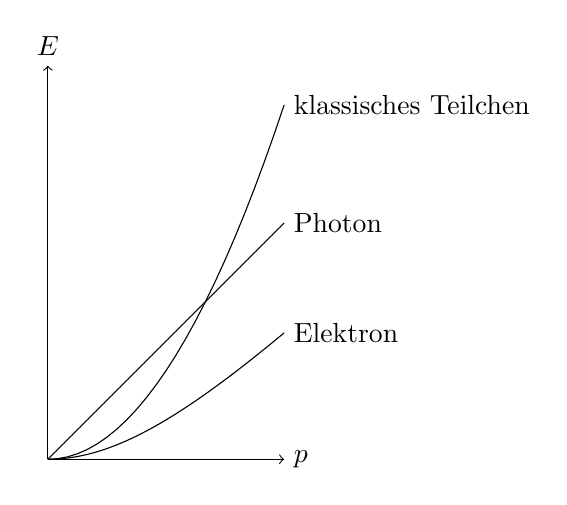
\begin{tikzpicture}[scale=2]
		\draw[->] (0, 0) -- ++(1.5, 0) node[right] {$p$};
		\draw[->] (0, 0) -- ++(0, 2.5) node[above] {$E$};
		\draw[domain=0:1.5] plot (\x, {\x}) node[right] {Photon};
		\draw[domain=0:1.5] plot (\x, {sqrt(1+\x^2) - 1}) node[right] {Elektron};
		\draw[domain=0:1.5] plot (\x, {\x^2}) node[right] {klassisches Teilchen};
	\end{tikzpicture}
	\caption{%
		Plot für die verschiedenen Teilchen. Für diesen Plot habe ich $c = h =
		1$ sowie für das Elektron $E_0 = m = 1$ gesetzt.
	}
	\label{fig:2-tikz}
\end{figure}

\begin{figure}
	\centering
	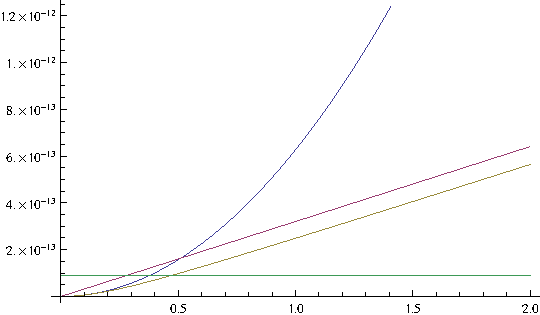
\includegraphics[width=.85\textwidth]{H2-Plot.pdf}
	\caption{%
		Plot der Energien für verschiedene Teilchen. In blau ist das klassische
		Elektron, in violett das Photon und in gelb das Elektron. In grün die
		Energie des Photons zur Compton-Wellenlänge. Auf der Ordinate ist der
		Impuls $p$ in $\si{\mega\electronvolt}/c$, auf der Abszisse die
		kinetische Energie $E$ in $\si\joule$.
	}
	\label{fig:2-mathematica}
\end{figure}

Für kleine Impulse sind die relativistische und die klassische Formel sehr nah
beieinander, wie zu erwarten ist.

\subsection{Compton-Wellenlänge}

Die Wellenzahl $k$ zur Compton-Wellenlänge ist:
\[
	k_\text{C} = \frac{2\piup}{\lambda_\text{C}} = \SI{2.84e12}{\radian\per\meter}
\]

Der Impuls dazu ist:
\[
	p_\text{C} = \hbar k_\text{C} = \SI{3.00e-22}{\kilogram\meter\per\second}
\]

Und die Energie:
\[
	E_\text{C} = cp_\text{C} = \SI{2.99e-22}\joule = \SI{.561}{\mega\electronvolt}
\]

Den Wert für $p_\text{C}$ habe ich nicht in Abbildung \ref{fig:2-mathematica}
eingezeichnet, da ich nicht weiß, wie in Mathematica eine vertikale Linie
eingefügt wird. Sie sollte aber bei \num{.56} liegen.

%%%%%%%%%%%%%%%%%%%%%%%%%%%%%%%%%%%%%%%%%%%%%%%%%%%%%%%%%%%%%%%%%%%%%%%%%%%%%%%
%            Atomares Magnetfeld, Kernmoment und Hyperfeinstruktur            %
%%%%%%%%%%%%%%%%%%%%%%%%%%%%%%%%%%%%%%%%%%%%%%%%%%%%%%%%%%%%%%%%%%%%%%%%%%%%%%%

\section{Atomares Magnetfeld, Kernmoment und Hyperfeinstruktur}
\label 3

\subsection{Magnetfeld am Ort des Protons}

Das Gesetz von Biot-Savart ist:
\begin{equation}
	\label{eq:biot-savart}
	\vec B\del{\vec x}
	= \frac{\mu_0}{4\piup} \int \dif{^3x'} \,
	\vec j\del{\vec x'} \times \frac{\vec x - \vec x'}{\abs{\vec x - \vec x'}}
\end{equation}

Ich nehme an, dass das Elektron wie eine Ringladung um das Proton verteilt ist,
damit ich ein zeitlich konstantes Magnetfeld erhalte.
\[
	\varrho(r, \phi, z)
	= \frac{e}{2\piup a_0} \delta(r - a_0) \delta(z)
\]

Mit dem Ansatz „Coulomb-Anziehung wirkt als Zentripetalkraft“ erhalte ich die
Geschwindigkeit:
\[
	\frac{1}{4\piup\varepsilon_0} \frac{e^2}{a_0^2} = m_\text{e} \frac{v_0^2}{a_0}
	\iff
	v_0 = \sqrt{\frac{1}{4\piup\varepsilon_0} \frac{e^2}{a_0 m_\text{e}}}
\]

Das Geschwindigkeitsfeld ist:
\[
	\vec v\del{\vec x} = v_0 \ev_\phi
\]

Somit ist die Stromdichte:
\[
	\vec j\del{r, \phi, z} = \varrho(r, \phi, z) \vec v\del{\vec x}
\]

Dies setze ich in \eqref{eq:biot-savart} ein:
\begin{align*}
	\vec B\del{\vec 0}
	&= \frac{\mu_0}{4\piup}
	\int_{-\infty}^\infty \dif z
	\int_0^{2\piup} \dif \phi'
	\int_0^\infty \dif r' \, r'
	\vec j\del{\vec x'} \times \frac{\vec 0 - \vec x'}{\abs{\vec 0 - \vec x'}} \\
	\intertext{%
		Das Integral über $r'$ führe ich aus. Dadurch werden nur alle $r'$ auf
		$a_0$ gesetzt. Außerdem schreibe ich die Vektoren aus.
	}
	&= - \frac{\mu_0}{4\piup}
	\int_{-\infty}^\infty \dif z
	\int_0^{2\piup} \dif \phi' \,
	a_0
	\frac{e}{2\piup a_0} \delta(z) v_0 \ev_\phi
	\times \frac{\vec x'}{a_0} \\
	&= - \frac{\mu_0}{4\piup} \frac{e}{2\piup a_0} v_0
	\int_0^{2\piup} \dif \phi' \,
	\ev_{\phi'}
	\times \begin{pmatrix}
		a_0 \cos\del{\phi'} \\
		a_0 \sin\del{\phi'} \\
		0
	\end{pmatrix} \\
	\intertext{%
		Das Kreuzprodukt liefert gerade $-1$.
	}
	&= \frac{\mu_0}{4\piup} \frac{e}{2\piup} v_0
	\int_0^{2\piup} \dif \phi' \,
	\ev_z \\
	\intertext{%
		Da nichts mehr von $\phi'$ abhängt, liefert diese Integration nur noch
		einen Faktor $2\piup$.
	}
	&= \frac{\mu_0}{4\piup} e v_0 \ev_z \\
	&= \frac{\mu_0}{4\piup} e^2 \sqrt{\frac{1}{4\piup\varepsilon_0} \frac{1}{a_0 m_\text{e}}} \ev_z
\end{align*}

Das Magnetfeld zeigt also – wie mit der rechten-Hand-Regel auch anschaulich zu
sehen – senkrecht zur Rotationsebene nach oben.

Von den Einheiten haut dies allerdings nicht hin, ich muss noch mit $a_0^{-2}$
multiplizieren, damit als Einheit Tesla herauskommt. Dann ist der Wert:
\[
	\vec B\del{\vec 0} = \SI{12.5}\tesla
\]

Wenn die Coulomb-Kraft zwischen zwei Nukleonen $\SI{150}\newton$ ist, dann ist
ein derart starkes Magnetfeld nicht weiter verwunderlich.

\subsection{Magnetisches Dipolmoment}

Für den Drehimpuls gilt:
\[
	\vec L
	= \vec r \times \vec p
	= m_\text{p} r_\text{p} v_\text{p} \ev_z
	= \underbrace{m_\text{p}^{} r_\text{p}^2}_{\Theta_\text{p}} \vec \omega
	\overset != \frac\hbar2 \ev_z
\]

Ich gehe davon aus, dass die Ladungsdichte ein dünner Ring um das Zentrum ist.
Der Strom durch eine $\ev_z \wedge \ev_\rho$ Ebene ist:
\[
	\vec I = e \frac{\omega}{2\piup} \ev_\phi
\]

Dies muss der Fall sein, weil die Integration nach der Zeit $t$ um eine ganze
Periode gerade die Ladung $e$ geben muss:
\[
	Q = \int_0^{\frac\omega{2\piup}} \dif t \, I = e
\]

Das magnetische Moment ist:
\[
	\vec\mu_\text{p}
	= \half I \oint_0^{2\piup} \vec x \times \vec{\dif l}
	= \half I \oint_0^{2\piup r_\text{p}} \dif \phi \, r_\text{p} \ev_z
	= \half e \frac{\omega}{2\piup} r_\text{p}^2 \oint_0^{2\piup} \dif \phi \, \ev_z
	= \half e \omega r_\text{p}^2 \ev_z
\]

Nun soll gerade $\vec L = \hbar \ev_z /2$ sein. Daher:
\[
	\vec \omega = \frac{\hbar}{2 m_\text{p}^{} r_\text{p}^2} \ev_z
\]

Somit ist das magnetische Moment:
\[
	\vec\mu_\text{p} = \frac{e \hbar}{4 m_\text{p}} \ev_z
\]

Nun noch einen Zahlenwert:
\[
	\vec\mu_\text{p} = \SI{2.9e-10}{\ampere\meter\squared}
\]

\subsection{Hyperfeinstruktur}

Die Energiedifferenz ist:
\[
	\Deltaup E = 2 B m = \SI{6.32e-26}\joule
\]

Die Frequenz dazu ist:
\[
	\nu_\text{HFS} = \frac{\Deltaup E}{h} = \SI{9.54e7}\hertz
\]

Mit einem Faktor \num{5.6} multipliziert ergibt dies gerade mal
\SI{530}{\mega\hertz}, und nicht die benötigten \SI{1.4}{\giga\hertz}. Da fehlt
also noch gut ein Faktor \num{2.5} irgendwo.

%%%%%%%%%%%%%%%%%%%%%%%%%%%%%%%%%%%%%%%%%%%%%%%%%%%%%%%%%%%%%%%%%%%%%%%%%%%%%%%
%                            Stern-Gerlach-Versuch                            %
%%%%%%%%%%%%%%%%%%%%%%%%%%%%%%%%%%%%%%%%%%%%%%%%%%%%%%%%%%%%%%%%%%%%%%%%%%%%%%%

\section{Stern-Gerlach-Versuch}
\label 4

\subsection{Skizze}

Der Versuchsaufbau ist in Abbildung \ref{fig:stern-gerlach-skizze} gezeigt.

\begin{figure}
	\centering
	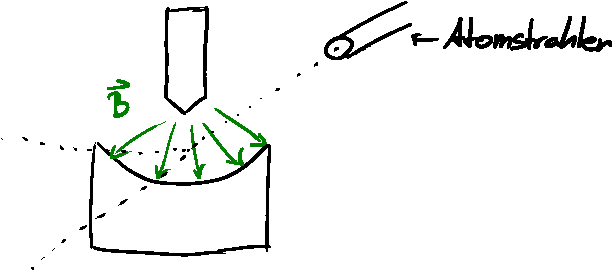
\includegraphics{H4-Skizze-crop.pdf}
	\caption{Aufbau des Stern-Gerlach-Experiments}
	\label{fig:stern-gerlach-skizze}
\end{figure}

Man wählt eine derartige Feldkonfiguration, damit es ein inhomogenes Feld und
somit ein $\od Bz \neq 0$ gibt. Ein homogenes Magnetfeld übt auf einen Dipol
ausschließlich ein Drehmoment aus. Für die Beobachtbarkeit ist es allerdings
wichtig, dass auch eine Kraft auf den Schwerpunkt ausgeübt wird, dies geht nur
mit einem inhomogenen Magnetfeld.

\subsection{Ablenkende Kraft}

Die potentielle Energie ist $V = - \inner{\vec \mu}{\vec B}$. Der negative Gradient gibt die Kraft:
\[
	\vec F
	= - \vnabla V
	= \vnabla \inner{\vec \mu}{\vec B}
\]

Unter der Annahme, dass das Magnetfeld nur entlang der $z$-Richtung variiert und $\vec \mu$ konstant ist, erhalte ich:
\[
	F_z = \inner{\vec \mu}{\dod{\vec B}z}
\]

Nach der klassischen Physik wäre zu erwarten, dass die magnetischen Momente
$\vec \mu$ thermisch verteilt sind, also im Mittel $\vec 0$ und isotrop. Daher
sollte die Ablenkung, die proportional zu $\mu$ ist, im Mittel null sein. Auf
dem Schirm ist ein (eventuell Gaußscher) Peak zu erwarten.

Im Experiment zeigen sich allerdings zwei Peaks. Daher gibt es für das
magnetische Moment nur zwei mögliche Zustände: $\mu = \pm \abs{\tilde\mu}$.
Diese können allerdings isotrop im Raum verteilt sein. Damit wird das
Vorzeichen eigentlich auch nicht gebraucht, weil es nur einer Rotation um
$\SI\pi\radian$ entspricht.

\subsection{Magnetisches Moment der Atome}

Die Kraft $F_z$ wirkt für die Zeit, die das Teilchen braucht, um den Magnet zu passieren:
\[
	t = \frac{l_1}{v_x}
\]

In dieser Zeit wirkt die Beschleunigung $a_y = F_z/M$. Somit ist die Auslenkung
direkt hinter dem Magneten:
\[
	d_z = \half a_z t^2
\]

Danach fliegt das Atom noch eine Zeit $t_2 = l_2/v_x$ mit der Geschwindigkeit
$v_z = a_z t_2$. Das gemessene $\delta_z$ ist die Kombination aus diesen beiden
Termen.

Zusammen mit der Kraft also:
\[
	\delta_z = \frac{\inner{\vec \mu}{\dod{\vec B}z}}{M} \del{\half \del{\frac{v_x}{l_1}}^2 + \frac{l_1l_2}{v_x^2}}
\]

Umgeformt:
\[
	\mu_z = \frac{d_z M}{\dod{B}z} \del{\half \del{\frac{v_x}{l_1}}^2 + \frac{l_1l_2}{v_x^2}}^{-1}
	= \SI{3.73e-22}{\ampere\meter\squared}
\]

Von den Einheiten her stimmt dies, allerdings ist dies deutlich kleiner als das
magnetische Moment des Protons, das in Aufgabe \ref 3 bestimmt worden ist.

%%%%%%%%%%%%%%%%%%%%%%%%%%%%%%%%%%%%%%%%%%%%%%%%%%%%%%%%%%%%%%%%%%%%%%%%%%%%%%%
%                                    Ende                                     %
%%%%%%%%%%%%%%%%%%%%%%%%%%%%%%%%%%%%%%%%%%%%%%%%%%%%%%%%%%%%%%%%%%%%%%%%%%%%%%%

\IfFileExists{\bibliographyfile}{
	%\bibliography{\bibliographyfile}
}{}

\end{document}

% vim: spell spelllang=de
